\documentclass[conference]{IEEEtran}
\IEEEoverridecommandlockouts

\usepackage{cite}
\usepackage{amsmath,amssymb,amsfonts}
\usepackage{graphicx}
\usepackage{textcomp}
\usepackage{xcolor}
\usepackage{booktabs}
\usepackage{multirow}
\usepackage{url}
\usepackage{microtype}
\usepackage{nicefrac}
\usepackage{xspace}
\usepackage[hidelinks]{hyperref}

\graphicspath{{../figures/}}

\newcommand{\PCSP}{\textsc{pcsp}\xspace}
\newcommand{\eg}{\textit{e.g.}\xspace}
\newcommand{\ie}{\textit{i.e.}\xspace}
\newcommand{\etal}{\textit{et al.}\xspace}

% ---------------------------------------------------------------
\title{One Policy, Infinite NPCs:\\
A Vision for Scalable Persona-Conditioned NPC Control\\
in Life Simulation Games}

\author{%
  \IEEEauthorblockN{Anonymous Author(s)}
  \IEEEauthorblockA{Anonymous Institution\\
    anonymous@institution.edu}
}

\begin{document}
\maketitle

% ---------------------------------------------------------------
\begin{abstract}
Life simulation games require hundreds to thousands of non-player characters (NPCs)
that each behave consistently with a distinct personality across an entire play
session. Current approaches---hand-authored behavior trees, per-character RL
policies, unsupervised skill discovery, and LLM-as-policy---each fail on one or
more of the four axes that matter for practical deployment: persona consistency,
natural-language controllability, zero-shot generalization, and real-time inference.
We argue that \emph{persona-conditioned shared policies}---a single RL policy
conditioned on frozen LLM embeddings of free-form persona descriptions---represent
a promising architectural direction that can satisfy all four axes simultaneously.
To support this argument we introduce \PCSP (Persona-Conditioned Shared Policy),
an early proof-of-concept combining frozen LLM encoding, LoRA projection,
FiLM conditioning, and a PPO + InfoNCE consistency + KL diversity co-training
objective. On a 300-persona life-simulation benchmark, \PCSP achieves zero-shot
persona identification 11$\times$ above chance, Spearman $\rho\!=\!0.73$
semantic-behavioral alignment, and 22$\times$ faster inference than LLM-as-policy.
We then lay out a concrete research agenda---covering dynamic personas, social
emergence, long-horizon memory, richer environments, human evaluation, and
authoring tools---for the community to build on this direction.
\end{abstract}

\begin{IEEEkeywords}
game AI, NPC personalization, reinforcement learning, persona conditioning,
large language models, life simulation
\end{IEEEkeywords}

% ---------------------------------------------------------------
\section{Introduction}
\label{sec:intro}

Modern life simulation games---\textit{The Sims}, \textit{Animal Crossing},
\textit{inZOI}, and emerging open-world titles---place NPCs at the center of
the player experience. For these games to feel alive, each NPC must behave
consistently with a distinct personality: the gregarious chef and the reclusive
artist should pursue the same biological needs through recognizably different
activity patterns, social approaches, and daily rhythms. At scale---hundreds to
thousands of NPCs per game world---this creates a fundamental challenge that
current game AI architectures were not designed to address.

\subsection{The NPC Personalization Scaling Gap}

\paragraph{Behavior trees} remain the industrial standard~\cite{yannakakis2018ai}.
A skilled designer hand-crafts decision logic for each character archetype.
This produces believable, predictable NPCs, but authoring cost scales linearly
with character count, and trees are brittle outside authored scenarios.
Ten thousand distinct NPC personalities require ten thousand hand-crafted trees.

\paragraph{Per-NPC RL} appears to offer automation: train a separate policy for
each persona. In principle this allows unlimited characters with arbitrary
behaviors. In practice, memory and training cost also scale linearly, and each
new persona requires a full retraining cycle---a prohibitive expense for
live-service games that regularly introduce new characters.

\paragraph{LLM-as-policy} methods~\cite{park2023generative,wang2023voyager,yao2023react}
achieve rich, natural-language-grounded persona expression by querying a language
model at every decision step. This works well in offline or turn-based contexts,
but current LLMs require 43--500\,ms per inference
call~\cite{achiam2023gpt4},
which exceeds the 16--33\,ms per-frame budget of real-time game simulations.
Generative Agents~\cite{park2023generative} sidestep this by operating on
minute-resolution plans rather than per-frame actions, which suits narrative
simulation but cannot drive moment-to-moment NPC movement and activity selection.

\paragraph{Unsupervised skill discovery} (DIAYN~\cite{eysenbach2018diayn},
CIC~\cite{laskin2022cic}) learns a shared policy conditioned on latent skill codes,
achieving behavioral diversity without per-character training. But the codes carry
no semantic content. A game designer cannot specify ``this NPC should be agreeable
and fitness-oriented'' by selecting a latent index.
Natural-language controllability is not part of the design.

\subsection{A Promising Architectural Direction}

We argue that the solution lies in a different decomposition: \emph{compute a
rich persona representation once per NPC, then condition a single lightweight
policy on that representation at every step}.

The key enabler is the modern LLM embedding space. A frozen language model maps
free-form persona descriptions to dense vectors that capture semantic
relationships among personalities. A shared policy conditioned on these
embeddings can generalize to \emph{any} persona a designer writes, without
retraining, because the continuous embedding space provides coverage of the
entire personality manifold. At inference time, the LLM is called once per NPC
lifetime; the policy network---at most a few hundred kilobytes---runs at full
game speed.

This architectural direction, which we call \emph{persona-conditioned shared
policies}, is not yet mature. The design space of embedding methods, conditioning
architectures, training objectives, and evaluation protocols remains largely
unexplored. The goal of this paper is threefold: (1)~articulate why this
direction is worth pursuing, (2)~present an early concrete instance (\PCSP) as
an existence proof, and (3)~identify the research questions that must be answered
to make the approach viable at game production scale.

\subsection{Paper Contributions}

\begin{enumerate}
  \setlength\itemsep{2pt}
  \item \textbf{Research agenda}: We identify persona-conditioned shared policies
    as an underexplored architectural direction and lay out six concrete open
    problems (\S\ref{sec:agenda}).
  \item \textbf{\PCSP}: An early proof-of-concept combining frozen
    Qwen3-0.6B-Embedding, LoRA projection, FiLM conditioning, and a
    PPO + InfoNCE + KL co-training objective (\S\ref{sec:method}).
  \item \textbf{Initial evidence}: On a 300-persona life-simulation benchmark,
    \PCSP achieves zero-shot persona identification 11$\times$ above chance,
    Spearman $\rho\!=\!0.73$ semantic-behavioral alignment, and 22$\times$
    faster inference than LLM-as-policy (\S\ref{sec:evidence}).
  \item \textbf{Evaluation agenda}: A proposal for metrics and benchmarks suited
    to persona fidelity evaluation beyond task reward (\S\ref{sec:evalagenda}).
\end{enumerate}

% ---------------------------------------------------------------
\section{Why Current Paradigms Fall Short}
\label{sec:paradigms}

Table~\ref{tab:paradigms} evaluates six paradigms against the four axes that
matter for practical life-simulation NPC deployment.

\begin{table}[t]
  \centering
  \small
  \caption{Paradigm comparison. \checkmark\,= satisfied, $\times$ = not
    satisfied, $\triangle$ = partially satisfied.}
  \label{tab:paradigms}
  \setlength{\tabcolsep}{3pt}
  \begin{tabular}{lcccc}
    \toprule
    Paradigm &
      \parbox{1.4cm}{\centering Persona\\consist.} &
      \parbox{1.2cm}{\centering NL\\control.} &
      \parbox{1.3cm}{\centering Zero-shot\\gen.} &
      \parbox{1.1cm}{\centering Real-time\\($<$5\,ms)} \\
    \midrule
    Behavior trees           & $\triangle$ & $\times$   & $\times$   & \checkmark \\
    Goal-cond.\ RL           & $\times$    & $\times$   & $\times$   & \checkmark \\
    Lang-cond.\ RL           & $\triangle$ & \checkmark & $\triangle$& \checkmark \\
    Skill discovery          & $\triangle$ & $\times$   & $\times$   & \checkmark \\
    Per-NPC RL               & \checkmark  & $\times$   & $\times$   & \checkmark \\
    LLM-as-policy            & \checkmark  & \checkmark & \checkmark & $\times$   \\
    \midrule
    \textbf{\PCSP (ours)}    & \checkmark  & \checkmark & \checkmark & \checkmark \\
    \bottomrule
  \end{tabular}
\end{table}

\paragraph{Goal-conditioned RL.}
UVFA~\cite{schaul2015uvfa} and HER~\cite{andrychowicz2017her} condition policies
on goal \emph{states}---what to achieve. Persona describes \emph{how to behave}:
two NPCs with identical needs but different personalities should fulfill them
through different activity sequences. Goal conditioning addresses the wrong axis
of variation and provides no natural-language interface.

\paragraph{Language-conditioned RL.}
BabyAI~\cite{chevalier2019babyai} conditions on natural-language
\emph{instructions} that change each episode.
Persona is a stable trait persisting over the NPC's lifetime; treating it as an
episode-level instruction discards the long-horizon consistency constraint.
Decision Transformer~\cite{chen2021decision} and similar sequence-modeling
approaches condition behavior on past returns or goals, but not on static identity
descriptors that must generalize zero-shot.

\paragraph{Unsupervised skill discovery.}
DIAYN~\cite{eysenbach2018diayn} and CIC~\cite{laskin2022cic} achieve behavioral
diversity via learned latent codes, but the codes carry no semantic content.
Generalizing to a new designer-specified persona requires solving an inverse
problem: find the latent code for ``an introverted accountant who prioritizes
learning.'' This is not supported by design.

\paragraph{LLM-as-policy.}
Generative Agents~\cite{park2023generative}, Voyager~\cite{wang2023voyager},
and ReAct~\cite{yao2023react} produce rich, persona-consistent behavior but at
43--500\,ms per step. Techniques such as action caching, plan reuse, and
smaller distilled models can reduce latency, but the fundamental tension---rich
language reasoning versus real-time step budgets---remains. Generalist agents
such as Gato~\cite{reed2022gato} demonstrate that a single model can handle
diverse tasks, but inference cost is similar.

\paragraph{Summary.}
No existing paradigm satisfies all four axes. The design space between
``fast but no NL control'' and ``NL control but too slow'' has not been
systematically explored. Persona-conditioned shared policies are a concrete
proposal for how to close this gap.

% ---------------------------------------------------------------
\section{\PCSP: A Concrete Early Instance}
\label{sec:method}

We present \PCSP as one specific point in the design space of persona-conditioned
shared policies. The components we have chosen are motivated by ablation evidence
but are not canonical; they represent a tractable first step, not a final
architecture.

\subsection{Environment: Mini-Inzoi}

\textit{Mini-Inzoi} is a PettingZoo AEC life-simulation environment on a
6$\times$6 grid with 4 agents, 8 bio-social needs (hunger, sleep, social,
leisure, hygiene, fitness, work, learning), and 12 discrete actions
(8 activity + 4 movement).
Observation $s\!\in\!\mathbb{R}^{20}$: position (2), time-of-day (1), needs (8),
and summaries of the other three agents (9).
Reward combines needs satisfaction, persona-aligned activity bonuses ($+0.5$ for
preferred actions), and social bonuses scaled by Big Five
compatibility~\cite{mccrae1992introduction}
($0.2 + 0.3 \times \text{cos-sim}(\text{BF}_i, \text{BF}_j)$).

\textbf{Persona dataset.}
300 persona texts are generated from 15 Big Five archetypes $\times$ 20
occupations (240 train / 60 zero-shot test).
Each text is a 2--3 sentence natural-language description that an NPC designer
might write for a new character.

\subsection{Persona Encoding}

Given persona text $p$, we compute a frozen LLM embedding
$\hat{e}_p \in \mathbb{R}^{1024}$ using Qwen3-0.6B-Embedding~\cite{qwen3embed}
(last-token pooling, L2-normalized).
This is computed once per NPC lifetime (14.6\,ms/persona), imposing negligible
runtime cost.

A learned LoRA projection~\cite{hu2022lora} ($r\!=\!16$,
$\text{lr}\!=\!10^{-4}$) maps $\hat{e}_p \to e_p \in \mathbb{R}^{64}$:
\[
  e_p = W_{\text{down}}^{\top}\,\sigma\!\left(W_{\text{up}}^{\top}\hat{e}_p\right),
  \quad W_{\text{up}} \in \mathbb{R}^{1024\times 512},\; W_{\text{down}} \in \mathbb{R}^{512\times 64}.
\]
The projection is necessary: raw Qwen3 embeddings over-represent occupational
similarity relative to personality similarity (salesperson$\leftrightarrow$executive:
0.61 vs.\ trainer$\leftrightarrow$blogger: 0.33).
After LoRA training, Spearman $\rho$ between embedding distance and behavioral KL
increases from 0.384 to 0.728 (\S\ref{sec:evidence}).

\subsection{FiLM-Conditioned Shared Policy}

The shared policy $\pi_\theta(a \mid s, e_p)$ is a 3-layer MLP (256-256-10)
where each hidden layer $h_\ell$ is conditioned via
FiLM~\cite{perez2018film}:
\[
  h_\ell' = \gamma_\ell(e_p) \odot h_\ell + \beta_\ell(e_p),
\]
with small linear networks $\gamma_\ell, \beta_\ell : \mathbb{R}^{64} \to \mathbb{R}^{256}$.
FiLM injects persona information at \emph{every} hidden layer, preventing the
persona signal from being diluted in deep representations.
An identical FiLM-conditioned value network $V_\phi(s, e_p)$ serves as the
critic. Total trainable parameters: 207K (excluding the frozen LLM).

\subsection{Co-Training Objective}

\begin{equation}
  \mathcal{L} = \mathcal{L}_{\text{PPO}} + \lambda_1 \mathcal{L}_{\text{consist}}
    + \lambda_2 \mathcal{L}_{\text{diverse}},
\end{equation}
with $\lambda_1\!=\!0.5$, $\lambda_2\!=\!0.1$ (PPO: $\gamma\!=\!0.99$,
$\epsilon\!=\!0.2$, GAE-$\lambda\!=\!0.95$, batch\,$=\!2048$~\cite{schulman2017ppo}).

\textbf{Consistency loss.}
A 2-layer GRU trajectory encoder $g_\phi(\tau) \in \mathbb{R}^{64}$
maps episode trajectories to L2-normalized embeddings.
InfoNCE~\cite{oord2018cpc} ($T\!=\!0.07$) aligns trajectory embeddings with
their originating persona embeddings:
\begin{equation}
  \mathcal{L}_{\text{consist}} = -\log
  \frac{\exp\!\bigl(\text{sim}(g_\phi(\tau), e_p)/T\bigr)}
       {\sum_{p' \in \mathcal{B}} \exp\!\bigl(\text{sim}(g_\phi(\tau), e_{p'})/T\bigr)}.
\end{equation}
This prevents the policy from producing trajectories that cannot be traced back
to their conditioning persona.

\textbf{Diversity loss.}
We maximize the expected KL divergence between policy distributions induced by
different personas at shared states:
\begin{equation}
  \mathcal{L}_{\text{diverse}} =
    -\mathbb{E}_{s,\, p \neq p'}\!\bigl[
      D_{\mathrm{KL}}\!\bigl(\pi_\theta(\cdot \mid s, e_p)
        \;\|\; \pi_\theta(\cdot \mid s, e_{p'})\bigr)
    \bigr],
\end{equation}
computed as a batched forward pass over $n\!=\!8$ sampled personas at 32 states.
This discourages behavioral collapse toward a persona-agnostic average.

\begin{figure}[t]
  \centering
  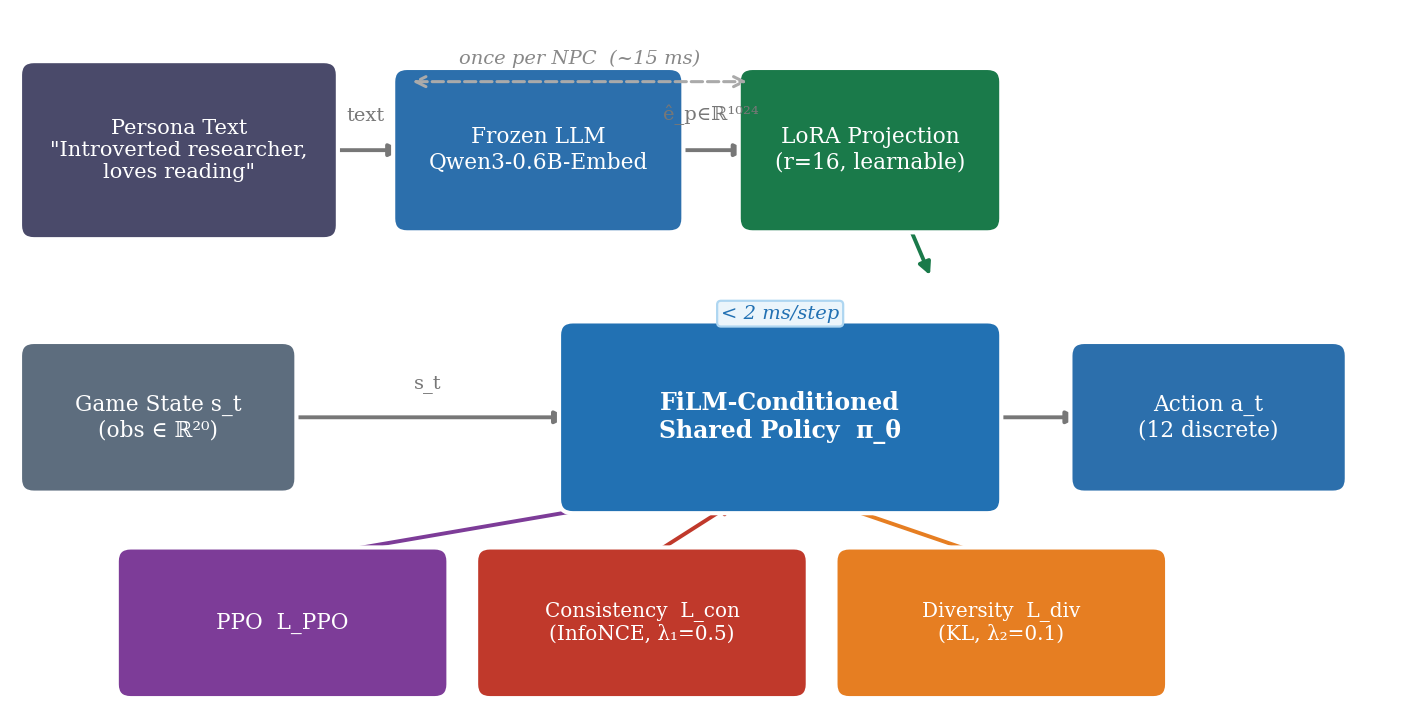
\includegraphics[width=\linewidth]{fig1_system.png}
  \caption{%
    \textbf{\PCSP system overview.}
    A frozen LLM encoder computes a once-per-NPC persona embedding.
    A learned LoRA projection adapts it to behavior space.
    The shared FiLM-conditioned policy runs at game speed ($<$2\,ms/step) and is
    trained with PPO + consistency + diversity co-objectives.}
  \label{fig:system}
\end{figure}

\subsection{What This Is Not}

\PCSP is a laboratory-scale proof-of-concept, not a production-ready NPC system.
The two Mini-Inzoi variants (6$\times$6 and 12$\times$12) are intentionally
minimal; the personas are synthetically generated; and human evaluation has not
been completed.
We present these results as evidence that the architectural direction is viable,
not as a claim that NPC personalization has been solved.

% ---------------------------------------------------------------
\section{Initial Evidence}
\label{sec:evidence}

We report experiments at two scales to test both the base design choices and
whether the architectural properties hold as the environment grows.

\subsection{Experimental Setup}

\textbf{v1 (base scale).}
Mini-Inzoi 6$\times$6, 4 agents, 300 personas (240 train / 60 zero-shot test).
All models train for 300 PPO iterations ($\approx$1.9M steps) on an NVIDIA
RTX 6000 Ada (49\,GB VRAM).
Baselines: \textbf{B1} No-Persona PPO; \textbf{B3} SBERT-conditioned policy
(\texttt{all-MiniLM-L6-v2}, 384-dim, frozen); \textbf{B4} DIAYN (random 64-dim);
\textbf{B5} LLM-as-policy (Qwen3-1.7B).

\textbf{v2 (expanded scale).}
Mini-Inzoi \textbf{12$\times$12, 16 agents, 500 personas} (400 train / 100
zero-shot test), 200 PPO iterations.
Same hyperparameters and evaluation protocol as v1.
The observation dimension expands to 56 (position 2, time 1, needs 8,
15 other agents $\times$ 3).
Random zero-shot chance is 1.0\% (1/100 test personas).

\subsection{Results}

Tables~\ref{tab:results_v1} and~\ref{tab:results_v2} show key metrics at each
scale. Figure~\ref{fig:learning} shows training reward curves at both scales.
Full ablation details appear in the supplementary.

\begin{figure}[t]
  \centering
  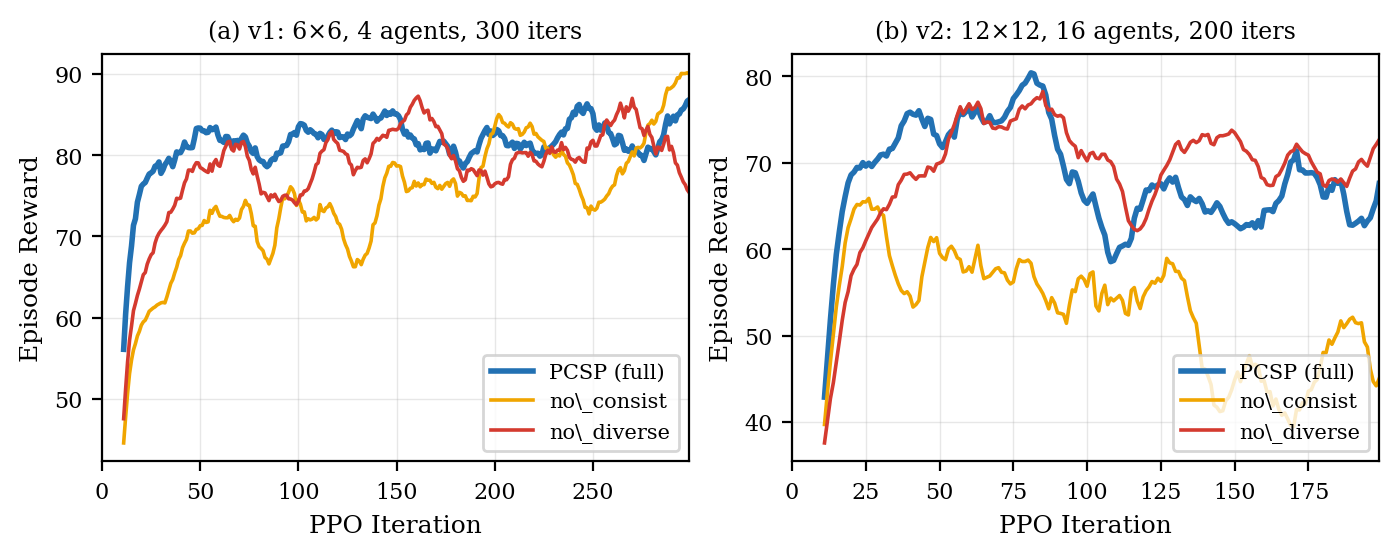
\includegraphics[width=\linewidth]{fig2_learning_v1v2.png}
  \caption{%
    \textbf{Training reward curves at two scales.}
    (a) v1 (6$\times$6, 4 agents, 300 iters).
    (b) v2 (12$\times$12, 16 agents, 200 iters).
    The diversity loss (no\_diverse) is the most critical ablation at both
    scales: its removal causes the largest reward drop and, more importantly,
    behavioral collapse (KL: v1 $0.39$, v2 $0.48$).
    The consistency loss (no\_consist) trades slightly higher reward for total
    loss of persona traceability.
  }
  \label{fig:learning}
\end{figure}

\begin{table}[t]
  \centering
  \small
  \caption{%
    \textbf{v1 results} (6$\times$6, 4 agents, 300 personas).
    ZS Acc: zero-shot $k$-NN accuracy on 60 unseen personas
    (random $\approx\!1.7\%$). $\rho$: Spearman (embedding dist.\ vs.\ KL).}
  \label{tab:results_v1}
  \setlength{\tabcolsep}{3pt}
  \begin{tabular}{lrrrr}
    \toprule
    Model & Reward $\uparrow$ & ZS Acc $\uparrow$ & $\rho$ $\uparrow$ & Lat.\ $\downarrow$ \\
    \midrule
    \textbf{\PCSP (full)}  & 83.4 & \textbf{0.193} & \textbf{0.728} & 1.97\,ms \\
    PCSP (no\_consist)     & 84.3 & 0.017*  & 0.638 & 2.03\,ms \\
    PCSP (no\_diverse)     & 76.8 & 0.147   & ---$^\dagger$ & 1.79\,ms \\
    B1 No-Persona          & 73.2 & ---     & ---   & 1.83\,ms \\
    B3 SBERT               & \textbf{86.2} & --- & --- & 1.88\,ms \\
    B5 LLM-policy          & ---  & ---     & ---   & 43.7\,ms \\
    \bottomrule
  \end{tabular}\\[2pt]
  {\footnotesize * Near-random (failure mode).
    $^\dagger$KL $\approx\!0.39$; $\rho$ not meaningful.}
\end{table}

\begin{table}[t]
  \centering
  \small
  \caption{%
    \textbf{v2 results} (12$\times$12, 16 agents, 500 personas).
    ZS Acc on 100 unseen personas (random $=\!1.0\%$).
    Lower absolute reward reflects the harder, larger environment.}
  \label{tab:results_v2}
  \setlength{\tabcolsep}{3pt}
  \begin{tabular}{lrrrr}
    \toprule
    Model & Reward $\uparrow$ & ZS Acc $\uparrow$ & $\rho$ $\uparrow$ & KL $\uparrow$ \\
    \midrule
    \textbf{\PCSP (full)}  & 64.2 & \textbf{0.023} & \textbf{0.725} & \textbf{5.40} \\
    PCSP (no\_consist)     & 50.1 & 0.000*  & 0.253 & 16.47$^\ddagger$ \\
    PCSP (no\_diverse)     & 71.6 & 0.013   & ---$^\dagger$ & 0.48 \\
    PCSP (concat)          & \textbf{74.8} & 0.027 & ---$^\dagger$ & 1.34 \\
    \bottomrule
  \end{tabular}\\[2pt]
  {\footnotesize * Exactly 0 (total failure). $^\dagger$KL too low; $\rho$ not meaningful.
    $^\ddagger$High KL without consistency reflects unstructured divergence, not persona alignment.}
\end{table}

\subsection{Key Observations}

Three findings from the v1 ablation study are replicated in v2, supporting
their generality across environment scales.

\textbf{Consistency loss is necessary for persona traceability.}
In v1, removing it drops zero-shot accuracy from 19.3\% to 1.7\% (random).
In v2, it drops from 2.3\% to exactly 0\% against a 1.0\% random baseline.
In both cases, trajectories carry no recoverable persona signal without this loss.

\textbf{Diversity loss prevents behavioral collapse.}
In v1, removing it reduces mean KL from 5.87 to 0.39 ($15\times$).
In v2, from 5.40 to 0.48 ($11\times$).
The collapse pattern is consistent: without this loss, the policy converges to
a persona-agnostic average regardless of environment size.

\textbf{Spearman $\rho$ is preserved across scales.}
\PCSP (full) achieves $\rho\!=\!0.728$ in v1 and $\rho\!=\!0.725$ in v2---a
difference of 0.003 despite a $4\times$ increase in grid area, $4\times$ more
agents, and $67\%$ more personas. This suggests that semantic-behavioral
alignment is a stable property of the architecture, not an artefact of the
minimal environment.

\subsection{Significance}

The absolute task reward and zero-shot accuracy are lower in v2, as expected for
a substantially harder environment with more test personas.
The key point is not the absolute numbers but the \emph{replication of
qualitative structure}: the same architectural decisions matter at both scales,
and the semantic-behavioral alignment property ($\rho \approx 0.73$) is
preserved. Figure~\ref{fig:zeroshot} shows the zero-shot distribution for v1;
the v2 pattern is qualitatively similar with narrower per-persona bars.
Figure~\ref{fig:kl} shows that the monotone relationship between persona
embedding distance and behavioral KL is virtually unchanged across the two
environments ($\rho\!=\!0.728$ vs.\ $0.725$), providing the clearest evidence
that semantic-behavioral alignment is a stable property of the architecture.
These results are \emph{early encouraging signs} that the direction is worth
pursuing at larger scale.

\begin{figure}[t]
  \centering
  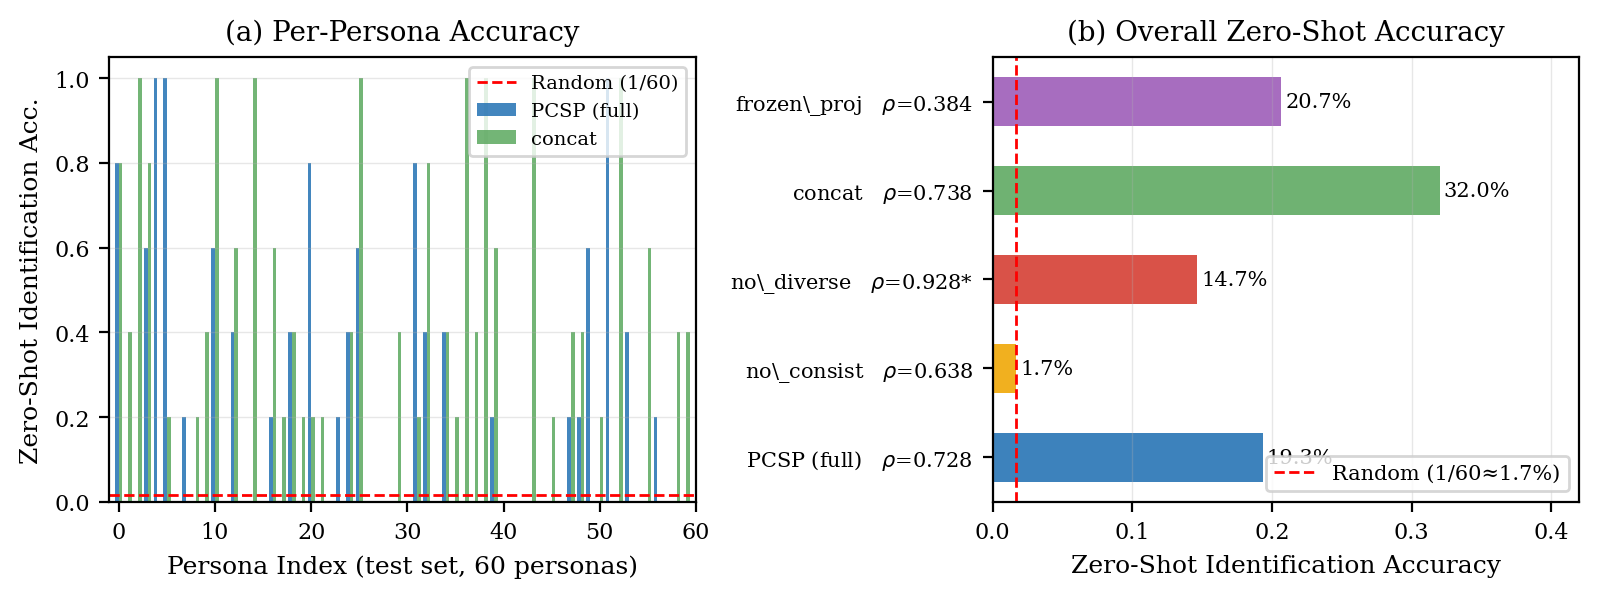
\includegraphics[width=\linewidth]{fig4_zeroshot.png}
  \caption{%
    \textbf{Zero-shot generalization on 60 unseen personas (v1).}
    \PCSP (full) achieves 19.3\% trajectory-to-persona identification;
    the red dashed line marks random chance (1.7\%).
    Removing the consistency loss collapses accuracy to 1.7\%.
    The v2 experiment (100 unseen personas) replicates this qualitative pattern.
  }
  \label{fig:zeroshot}
\end{figure}

\begin{figure}[t]
  \centering
  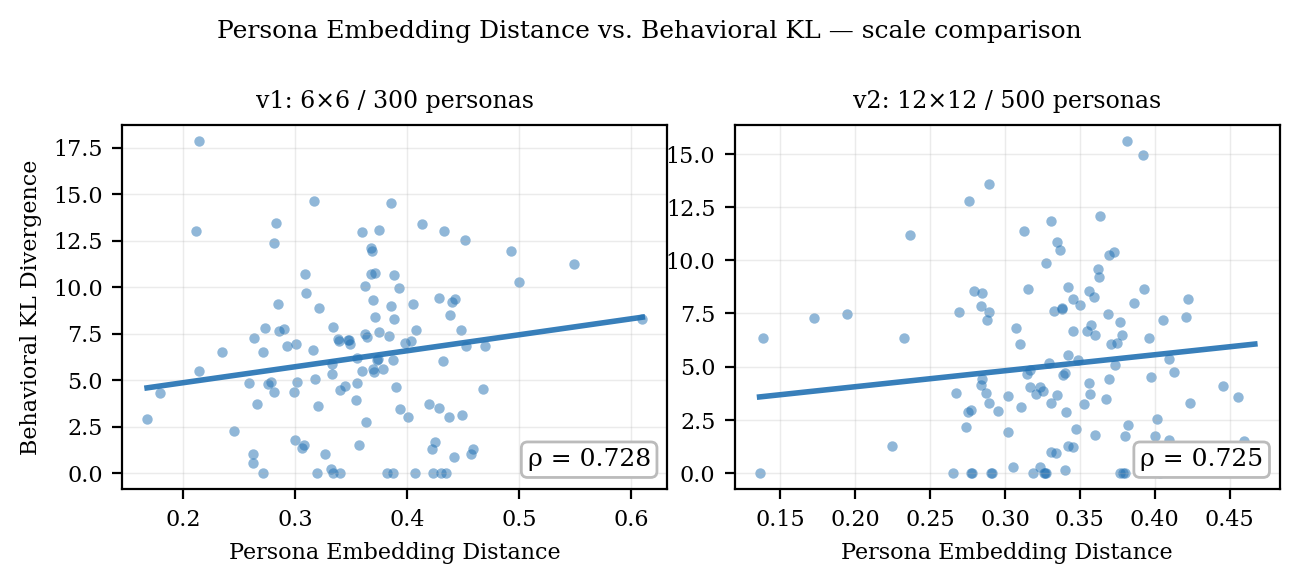
\includegraphics[width=\linewidth]{fig3_kl_v1v2.png}
  \caption{%
    \textbf{Persona embedding distance vs.\ behavioral KL divergence
    at two scales (PCSP full).}
    Left: v1 ($\rho\!=\!0.728$). Right: v2 ($\rho\!=\!0.725$).
    The monotone alignment between LLM semantic space and behavior space
    is preserved when moving to a 4$\times$ larger grid with 4$\times$
    more agents and 67\% more personas.
  }
  \label{fig:kl}
\end{figure}

% ---------------------------------------------------------------
\section{Research Agenda for Infinite NPCs}
\label{sec:agenda}

The results above are encouraging, but Mini-Inzoi is a deliberately minimal
environment. Reaching production-quality NPC personalization requires answering
six open research questions. We outline each with the core challenge and
candidate approaches.

\subsection{Dynamic Personas and Identity Evolution}

Current \PCSP encodes a static persona text computed once at NPC creation.
Real characters evolve: a traumatic in-game event should shift an NPC toward
neuroticism; forming a friendship should increase agreeableness over time.

The key challenge is \emph{representation}: how should an evolving personality
be maintained and encoded without expensive LLM calls at every update?
Candidate approaches include (a) maintaining a low-dimensional latent personality
state updated by a lightweight delta model at milestone events, (b) conditioning
the LoRA projection on recent interaction history via a rolling context encoder,
or (c) hierarchical persona representations that separate stable traits
(\eg conscientiousness) from volatile moods (\eg current frustration level).

\subsection{Socially Emergent Multi-Agent Behavior}

In multi-agent settings, personas interact: an introverted NPC paired with an
extroverted one may develop avoidance patterns; two agreeable NPCs may form
stable dyads. These emergent social structures are a major source of narrative
interest in life-simulation games.

Multi-agent RL methods such as MADDPG~\cite{lowe2017maddpg} and value
decomposition networks~\cite{sunehag2018vdn} provide starting points, as does
work on emergent compositional communication~\cite{mordatch2018emergence}.
The key challenge is designing reward structures that incentivize
persona-\emph{consistent} social patterns rather than converging to a single
globally optimal interaction style irrespective of individual personality.

\subsection{Long-Horizon Memory and Identity Persistence}

A believable NPC should remember a grudge from ten play sessions ago. Current
\PCSP has no episodic memory beyond the persona embedding and within-episode
trajectory. Connecting persona-conditioned behavior to long-horizon memory
architectures---transformer-based context~\cite{chen2021decision},
retrieval-augmented episodic memory~\cite{park2023generative}, or world
models~\cite{ha2018world}---is an open problem.

The persona-conditioned shared policy framework naturally separates \emph{who
this NPC is} (persona embedding, static) from \emph{what has happened to this
NPC} (episodic memory, dynamic). Developing architectures that condition behavior
on both, without expensive per-step LLM calls, is a key challenge.

\subsection{Richer Worlds and Engine Integration}

Mini-Inzoi's 6$\times$6 grid with 4 agents is a tractable starting point.
Scaling to commercial life-simulation density---larger worlds, more agents,
richer action spaces, continuous physics, asynchronous event streams---requires
rethinking both the environment interface and the policy architecture.

Melting Pot~\cite{leibo2021meltingpot} provides a suite of multi-agent social
scenarios at larger scale and is a natural next evaluation target.
Beyond simulation, integrating trained policies with commercial game engines
(Unreal Engine, Unity) as callable policy modules raises practical integration
challenges---latency stacking, state serialization, engine-side randomness---that
have received little academic attention.

\subsection{Human Evaluation for Persona Fidelity}

The ultimate judge of NPC believability is the player.
Automatic metrics (trajectory identification accuracy, behavioral KL,
Spearman $\rho$) are useful proxies for ablations but cannot capture whether a
player experiences an NPC as authentically ``introverted'' or ``conscientious.''

Designing psychometrically valid human evaluation protocols for NPC persona
fidelity is non-trivial. Existing personality assessment instruments (Big Five
questionnaires~\cite{mccrae1992introduction}) were designed for real humans.
Adapting methods from personality computing~\cite{vinciarelli2014survey} and
human-agent interaction to NPC personas---with controlled observer studies,
inter-rater agreement ($\alpha \geq 0.6$), and adequate sample sizes
($n \geq 100$)---is an important open methodological task.

\subsection{Authoring Tools for Game Designers}

For this research direction to reach production, it must interface with designers'
workflows. Designers author NPC personalities through prose, reference personality
frameworks, and iterate based on playtester feedback.
A persona-conditioned shared policy system should provide:
\begin{itemize}
  \setlength\itemsep{0pt}
  \item An interface for writing and previewing persona descriptions.
  \item Rapid feedback on the predicted behavioral effect of a persona change,
    without requiring a full retraining cycle.
  \item Diagnostic tools that explain \emph{why} an NPC is behaving as it does
    in terms the designer can act on.
  \item Control over the precision-recall trade-off between persona fidelity and
    task performance.
\end{itemize}
None of these tools exist in current RL-based NPC literature.
Addressing them connects the technical research agenda to design practice.

% ---------------------------------------------------------------
\section{Evaluation Agenda}
\label{sec:evalagenda}

Progress on the research agenda requires standardized evaluation protocols.
We propose the following minimum set of metrics for persona-conditioned NPC
research, beyond task reward.

\paragraph{Persona identification accuracy.}
Given a trajectory, can an observer (automated or human) identify which persona
generated it? We recommend reporting both in-distribution (training personas) and
zero-shot (held-out personas) $k$-NN accuracy. This measures how strongly behavior
reflects the conditioning signal.

\paragraph{Behavioral diversity.}
Mean pairwise KL divergence between action distributions conditioned on different
persona embeddings. Low values indicate behavioral collapse regardless of task
reward.

\paragraph{Semantic-behavioral alignment.}
Spearman $\rho$ between persona embedding cosine distances and pairwise
behavioral KL divergences. This measures whether the semantic structure of persona
space is faithfully reflected in behavior space---the key criterion for zero-shot
generalization. High $\rho$ with low KL variance indicates alignment without
meaningful diversity; both should be reported together.

\paragraph{Inference latency.}
GPU ms/step at batch size 1, with p95/p99 percentiles. The practical constraint
for real-time engine integration is typically $<$16\,ms/frame.

\paragraph{Human-rated believability.}
Observer ratings of persona consistency and character naturalness, aggregated with
inter-rater agreement (Krippendorff's $\alpha$). This is the ground-truth criterion
for production deployment and should not be deferred indefinitely.

We further advocate for a dedicated \emph{persona-conditioned NPC benchmark}---perhaps
an adaptation of Melting Pot~\cite{leibo2021meltingpot} with curated personality
profiles and standardized evaluation protocols---to enable reproducible comparison
across future methods.

% ---------------------------------------------------------------
\section{Limitations and Scope}
\label{sec:limits}

\PCSP's current limitations are significant and should calibrate how its results
are interpreted.

\textbf{Minimal environments.}
Both Mini-Inzoi variants (6$\times$6 / 4 agents and 12$\times$12 / 16 agents)
are far removed from commercial life-simulation complexity. While the v2
experiment shows that key architectural properties hold at larger grid scale,
continuous physics, longer time horizons, and richer action semantics remain
untested.

\textbf{Synthetic personas.}
All 300 personas are algorithmically generated from Big Five archetypes and
occupation templates. Whether the method works with designer-authored personas---with
all their nuance, inconsistency, and cultural specificity---is untested.

\textbf{No human evaluation.}
Zero-shot identification accuracy and Spearman $\rho$ are automated proxies.
We have not yet collected player judgments of persona fidelity. This is a
necessary step before drawing conclusions about perceived NPC believability.

\textbf{No engine integration.}
The policy runs in a Python simulation environment. Integration challenges with
commercial game engines remain unknown.

These limitations are not arguments against the research direction---they are
precisely the open problems that motivate \S\ref{sec:agenda}. We present them
explicitly to guard against overclaiming.

% ---------------------------------------------------------------
\section{Conclusion}
\label{sec:conclusion}

Life simulation games create a scaling challenge that the game AI field has not
yet systematically addressed: how to give hundreds to thousands of NPCs distinct,
consistent, and controllable personalities without proportional authoring or
inference cost. We have argued that \emph{persona-conditioned shared
policies}---a single RL policy conditioned on frozen LLM persona
embeddings---represent a promising architectural direction satisfying the four
axes that matter for practical deployment, and we have presented \PCSP as an
early proof-of-concept supporting this argument.

The central message is not that \PCSP solves NPC personalization. The central
message is: \emph{there exists a region of design space---combining language
semantics, shared policies, and behavioral regularization---where persona
consistency, zero-shot controllability, and real-time inference can coexist}.
Exploring that region systematically is a concrete and tractable research program.
We hope this paper motivates the community to take it up.

% ---------------------------------------------------------------
\bibliographystyle{IEEEtran}
\bibliography{refs}

\end{document}
